\chapter{\btagging Study}
\label{c:b_tagging_study}

Since the \tquark decays to a \W boson and a \bquark, the understanding of these decay products is important
in studies of \ttbar events. In particular, methods to identify jets coming from a \bquark, known as
\btagging, are commonly used to increase the efficiency of a signal selection. CMS has several algorithms for
\btagging: TrackCounting (High Efficiency) and TrackCounting (High Purity), JetBProbability; JetProbability;
SoftMuon; SoftMuonByPt; SoftMuonByIP3d; SimpleSecondaryVertex (High Efficiency); SimpleSecondaryVertex (High
Purity); CombinedSecondaryVertex; CombinedSecondaryVetexMVA. These algorithms produce a discriminator output
for each jet which indicates how likely it is to be a \b flavour jet. In all cases, a more positive
discriminator value indicates a jet that is more likely to be a \b flavour jet. Performance of the different
algorithms varies owing to the fact that they use different jet properties to produce their discriminators.


\section{\btagging algorithm descriptions}
\label{s:btagging_algorithm_descriptions}

\subsection*{Track Counting}
\label{ss:track_counting}
The simplest \btagging algorithm available in CMS is the track counting algorithms~\cite{CMS-PAS-BTV-09-001},
which positively identifies a \bjet if it contains N or more tracks with IP significance above some theshold
value. They function by ordering all good tracks in a jet by order of decreasing IP significance, with the
discriminator being the IP significance of the Nth track. The high efficiency version of this algorithm uses
N=2, i.e. the second track, and the high purity version uses N=3, i.e. the third track~\cite{CMS-AN-2005-041}.

\subsection*{Jet Probability}
\label{ss:jet_probability}
The jet probability algorithms~\cite{CMS-PAS-BTV-09-001} produce a discriminator based on the probability that
the set of tracks come from the primary vertex; a high probability would indicate that the jet is not a \bjet,
which would originate at a secondary vertex. These algorithms use all tracks as input and for each track
define an individual probability of coming from the primary vertex. By combining these probabilities, a jet
probability is produced, and the discriminator is the negative log of this confidence
level~\cite{CMS-AN-2005-041}. The jet B probability variant is based on the four most displaced tracks in the
jet, since the mean number of tracks in a b jet is approximately 5 and the reconstruction of tracks within
jets has an efficiency of approximately 0.8 in CMS~\cite{CMS-PAS-BTV-09-001}. The jet B probability in this
case is based on the confidence level that the four most displaced tracks originate from the primary vertex.

\subsection*{Soft Muon}
\label{ss:soft_muon}
The Soft Muon algorithms make use of global muons reconstructed in the vicinity of the reconstructed jet,
which may indicate a semi-leptonic decay of B hadrons to a muon~\cite{CMS-AN-2009-085}. Two soft muon
algorithms exist in CMS. The soft muon by \pt algorithm uses the relative \pt of the muon with respect to the
jet (\pt$_{rel}$), which is expected to be larger than muons in light flavour jets due to the large \bquark
mass~\cite{CMS-AN-2009-085, Ferro:2012tg}. A soft muon by IP algorithm also exists which uses the IP
significance of positive IP muons. In jets containing more than one muon, the muon with the highest
discriminator is used.

\subsection*{Simple Secondary Vertex}
\label{ss:simple_secondary_vertex}
The simple secondary vertex (SSV) algorithm uses the Adaptive Vertex Fitter to reconstruct the secondary
vertex~\cite{Frühwirth:1027031}. The discriminator is calculated based on the 3D decay length significance
(the ratio between the flight distance and the uncertainty on this value). If no secondary vertex is reconstructed, no discriminator is produced, meaning
that the effiency of this algorithm is limited to the maximum effiency of secondy vertex reconstruction
(approximately 65\%)~\cite{Chatrchyan:2012jua}. There are two variants of the simpmle secondary vertex algorithm: the
high effiency version uses vertices with at least two compatible tracks, whereas the high purity version uses
vertices with at least three tracks. Since this algorithm does not directly use track-based lifetime
parameters, it is less sensitive than other algorithms to tracker misalignment.

\subsection*{Combined Secondary Vertex}
\label{ss:combined_secondary_vertex}
The current CMS recommendation is to use the Combined Secondary Vertex (CSV) algorithm~\cite{Weiser:2006md}
for physics analyses. This algorithm reconstructs the event vertices using the Trimmed Kalman Vertex
Finder~\cite{Speer:927395}. This vertex finding algorithm fits tracks to a primary vertex after removing
incompatible tracks and applies cuts to these vertices in order to find a secondary vertex. The CSV algorithm
then combines track-based lifetime parameters, such as IP and flight distance significance, with secondary
vertex information to prouce a discriminator. The increased number of input parameters mean that even in
cases with no reconstructed secondary vertex, a discriminator can be produced, thereby increasing the maximum
efficiency compared to the SSV algorithms~cite{Chatrchyan:2012jua}. A variant of this algorithm in which a
multi-variate analysis (MVA) is used to combine the variables and produce a discriminator.

\section{Performance Comparison}
\label{s:performance_comparison}

Distributions of the discriminators produced by the above algorithms were created for a \ttbar \MADGRAPH Monte
Carlo simulation sample (/TTJets\_TuneZ2\_7TeV-madgraph-tauola/, produced in the Fall2011 production cycle
using CMSSSW version 44X). Comparison of discriminator distributions for the described algorithms were carried
out Figure~\ref{fig:CSV_discriminators} shows a comparison between the distributions obtained by the CSV
algorithm for the different jets present in the sample: \bjets, light jets (up, down and strange flavour:
\udsjets), gluon jets (\gjets) and charm flavour jets (\cjets). All distributions were normalised to unity in
order to facilitate shape comparision. Equivalent plots for other algorithms are included in
Figure~\ref{fig:all_algorithm_discriminators} in Appendix~\ref{ac:b_tagging_plots}. In all cases, it can be
seen that higher discriminator values were produced for \bjets than for \udsjets, \gjets and \cjets, as would
be expected.

\begin{figure}[hbtp]
   \centering
     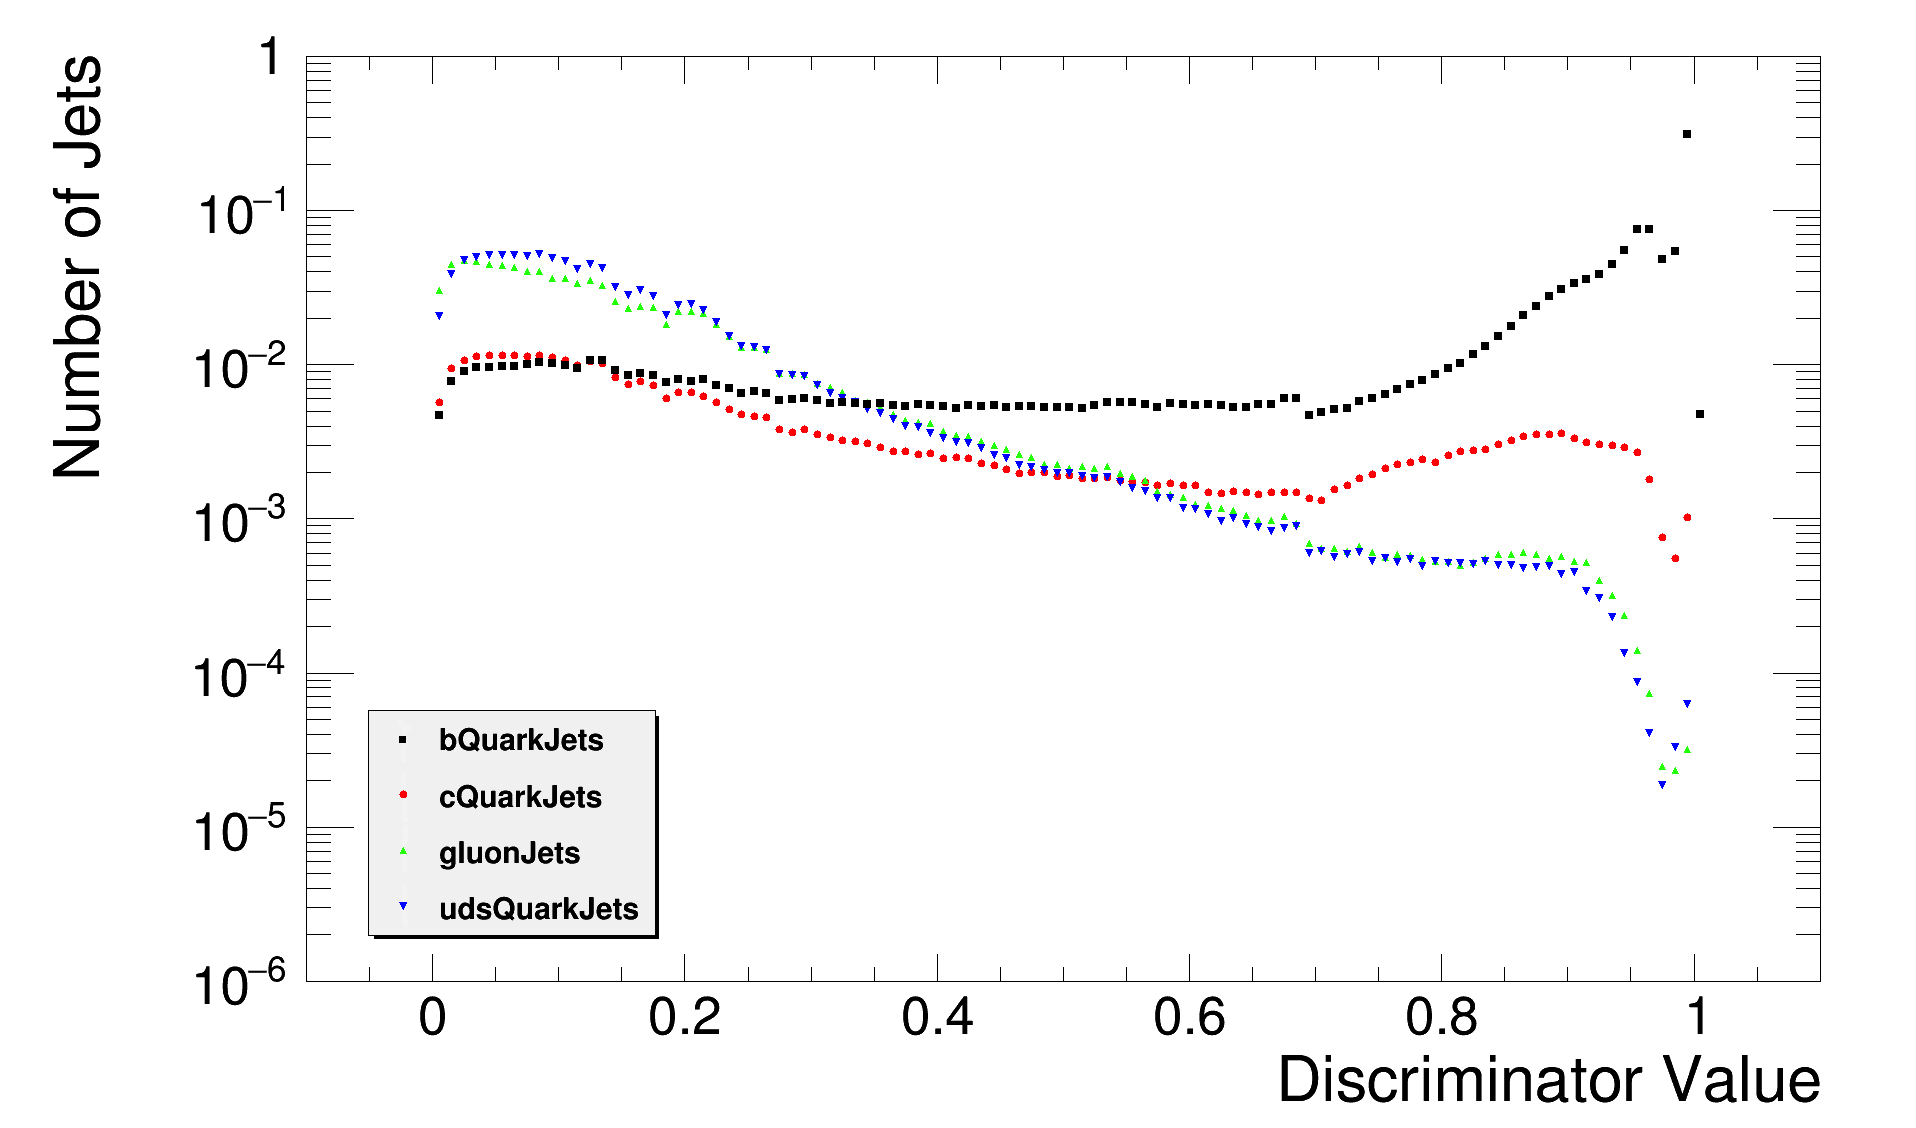
\includegraphics[width=\textwidth]{Chapters/04_Analysis/04a_BTags/Images/CombinedSecondaryVertex_norm_discriminator_combined}\\
     \caption[Discriminator values produced by the Combined Secondary Vertex algorithm after
     normalisation.]{Discriminator values produced by the Combined Secondary Vertex algorithm for all \bjets,
     \cjets, \gjets and \udsjets after normalisation.}
     \label{fig:CSV_discriminators}
\end{figure}

\section{Efficiency}
\label{s:efficiency}

Analyses in CMS make use of \btagging algorithms by placing cuts on the discriminators. The efficiency of a
cut can be defined as the ratio of number of jets passing the selection cut to the total number of jets before
the selection cut. In the case of the discriminator distributions produced here, cutting on a desired
discriminator value allows the efficiency of that cut to be found from the ratio of the area to the right of
the cut value to the total histogram area. The efficiency was calculated for cut values spanning the whole
range of discriminator values, thereby producing a plot of \btag efficiency as a function of cut value.
Figure~\ref{fig:CSV_jet_efficiencies} shows the \btag efficiency variation with cut value for the CSV
algorithm. In practice, the aim is to acheive a high \bjet efficiency and a low efficiency for all other jet
flavours, \ie towards the bottom right of the plot. It can be seen that the efficiency for \udsjets and \gjets
have similar increases in efficiencies with increasing cut value, owing to their similar discriminator
distributions in Figure~\ref{fig:CSV_discriminators}. The \cjet discriminator distribution has a noticeably
different shape, slightly similar to that of \bjets, in particular at low discriminator values. Therefore,
discriminator cuts show lower efficiencies for \bjets and higher efficiencies for \udsjets and \gjets, both
of which are undesireable trends. Equivalent plots for other algorithms can be found in
Figure~\ref{fig:all_algorithm_efficiencies} in Appendix~\ref{ac:b_tagging_plots}.

\begin{figure}[hbtp]
   \centering
     \includegraphics[width=\textwidth]{Chapters/04_Analysis/04a_BTags/Images/CombinedSecondaryVertex_nonBJetEfficiency_v_bJetEfficiency}\\
     \caption[Non \bjet efficiencies as a function of \bjet efficiency for the CSV algorithm.]{Non \bjet
     efficiencies as a function of \bjet efficiency for the CSV algorithm.}
     \label{fig:CSV_jet_efficiencies}
\end{figure}

\section{Algorithm Comparison}
\label{algorithm_comparison}

The performances of the various algorithms can be compared in Figure~\ref{fig:uds_eff_v_b_eff}.

\begin{figure}[hbtp]
   \centering
     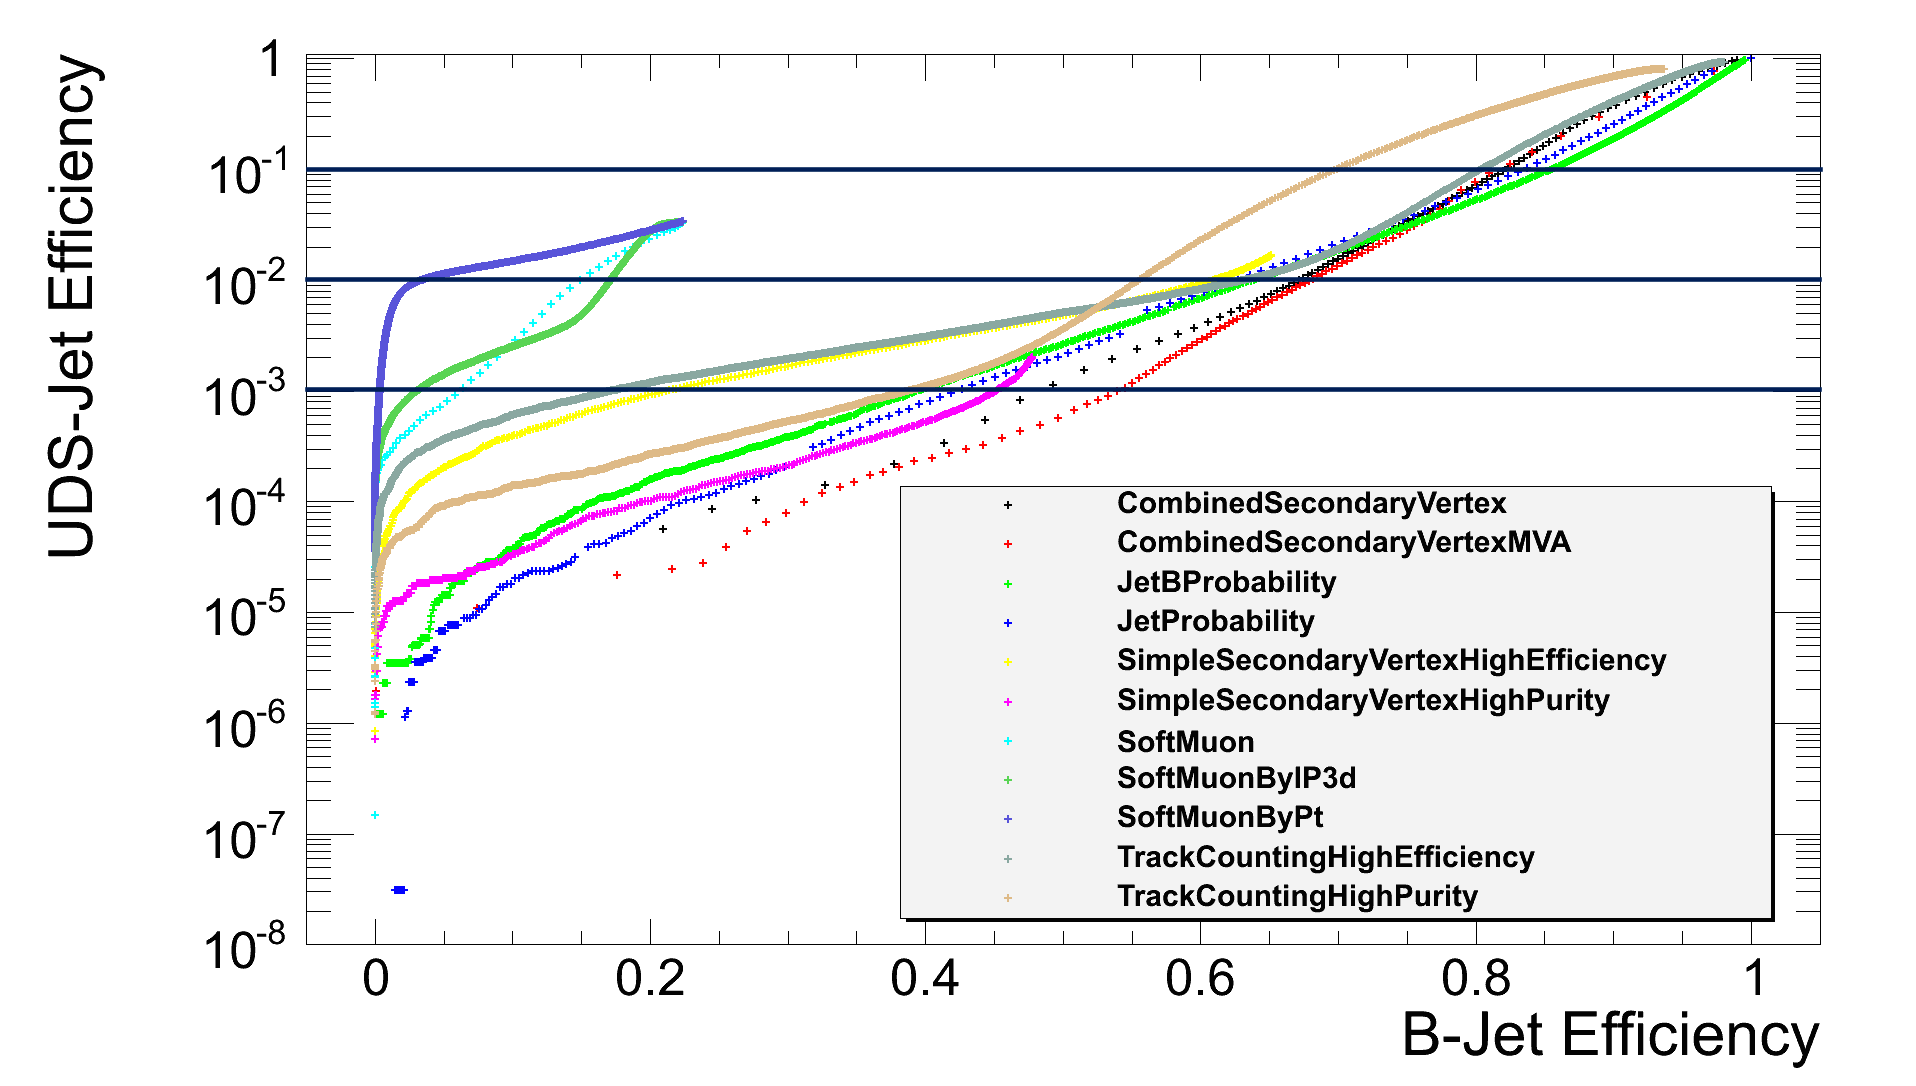
\includegraphics[width=\textwidth]{Chapters/04_Analysis/04a_BTags/Images/udsJetEfficiency_v_bJetEfficiency_withLegend_wp}\\
     \caption[udsjet efficiencies as a function of \bjet efficiencies for all algorithms.]{\udsjet
     efficiencies as a function of \bjet efficiencies for all algorithms.}
     \label{fig:uds_eff_v_b_eff}
\end{figure}

Once more, algorithms which reach closest to the lower right of the plot show better performance, according to
the requirements of high b jet efficiency and low light jet efficiency. It can be seen that not all algorithms
reach 100\% \bjet efficiency due to being inherently limited by their methods. For example, the soft muon
algorithms are limited by the muon identification efficiency within \bjets and also by the branching fraction
of B hadrons to muons. For instance, the soft muon algorithms all show low maximum \bjet efficiencies due to
the low B hadron semi-leptonic branching ratio to muon of approximately 11\% (or 20\% when further decays are
included such as b$\rightarrow$ c $\rightarrow$ l) \cite{Ferro:2012tg}. Similarly, the SSV algorithms are
limited by the efficiency of reconstructing a secondary vertex in the jet of approximately 65\%.

The 2011 and 2012 CMS recommended \btagger is the Combined Secondary Vertex with operating point discriminator
cuts of 0.244 (loose), 0.679 (medium) and 0.898 (tight) corresponding to 10\%, 1\% and 0.1\% light jet and
gluon jet efficiencies respectively. These cuts are indicated by the horizontal lines on
Figure~\ref{fig:uds_eff_v_b_eff}. It can be seen that for the tight and medium cuts, the CSV MVA algorithms
provides highest \bjet efficiency and lowest light jet efficiency, followed closely by the CSV algorithm.
The multiple variables that are used as input allow the CSV algorithm to produce higher efficiencies than the
SSV algorithms, while the MVA variant improves the slightly on correctly identifying jets from \bquarks. At
approximately 3\% light jet efficiency, there is a convergence of many algorithms that all provide similar
performance. At the loose working point also, many of the algorithms provide similar performance with \bjets,
with the JetProbability algorithms marginally outperforming the CSV algorithms TODO:NOT SURE WHY
JETPROBABILITY OUTPERFORMS HERE, BUT NEED TO ADD A SENTENCE EXPLAINING HERE.
